%% ΠΕΡΙΓΡΑΦΗ ΤΟΥ GOOGLE CALENDAR API
%% Σε αυτό το κεφάλαιο περιγράφεται το Google Calendar API
%% και το πως χρησιμοποιείται από το σύστημα για να πραγματοποιηθεί
%% η διαδικασία του συγχρονισμού.

\chapter{Google Calendar API}
Το Ημερολόγιο της Google είναι μια διαδικτυακή εφαρμογή που επιτρέπει στους χρήστες της να αποθηκεύουν και να διαχειρίζονται τα ραντεβού και τα συμβάντα τους σε ένα όμορφο περιβάλλον. Εκτός αυτού, υπάρχουν πολλές πρόσθετες δυνατότητες όπως ο συγχρονισμός ημερολογίου με κάποια άλλη εφαρμογή ή η κοινή χρήση ενός ημερολογίου από 
πολλά άτομα.

Όπως και με τα περισσότερα προϊόντα της Google παρέχονται εργαλεία με τα οποία μπορούν οι προγραμματιστές να επικοινωνήσουν και να λάβουν δεδομένα από τις υπηρεσίες της εταιρείας. Με 
αυτόν τον τρόπο είναι δυνατή η ανάπτυξη εφαρμογών οι οποίες διαχειρίζονται αυτά τα δεδομένα, διευκολύνοντας έτσι τον χρήστη.

\begin{figure}[h]
\centering
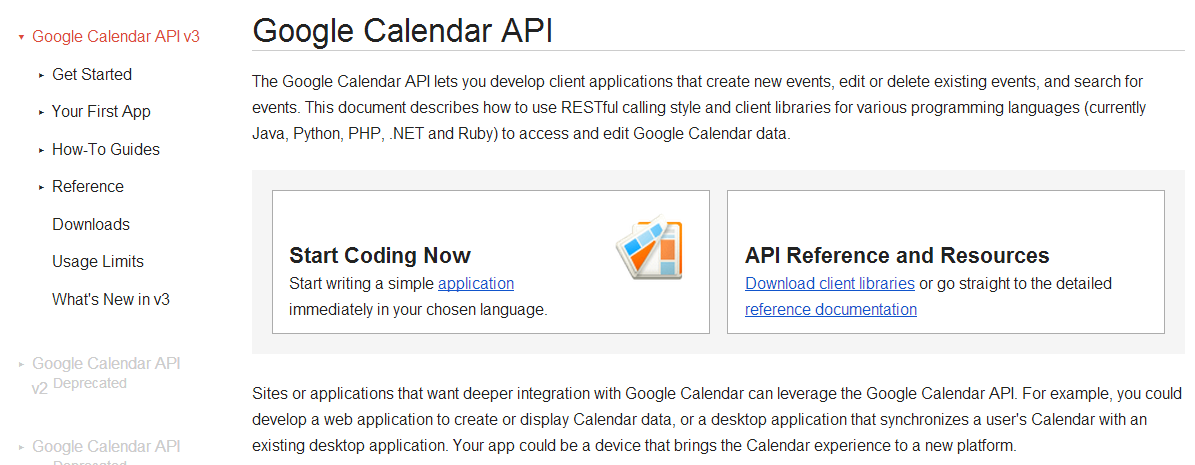
\includegraphics[width=150mm]{images/google-calendar-api.png}
\caption{Ιστότοπος περιγραφής του Google Calendar API.}
\label{google-calendar-api}
\end{figure}

Το Google Calendar API (Application Programming Interface) 
είναι μια πλατφόρμα διαχείρισης συμβάντων ενός ημερολογίου από την Google. Επιτρέπει στον προγραμματιστή να πραγματοποιήσει λειτουργίες προσθήκης, επεξεργασίας, διαγραφής και αναζήτησης συμβάντων μέσω ενός RESTful στυλ κλήσεων προς τον server.

Με την έννοια RESTful (Representional State Transfer) εννοείται ένας από τους πιο δημοφιλής τρόπους επικοινωνίας στον παγκόσμιο ιστό. Η επικοινωνία γίνεται με την χρήση ειδικών αιτήσεων προς τους servers οι οποίοι με την σειρά τους είναι σε θέση να τις επεξεργαστούν και να επιστρέψουν δεδομένα πίσω στους clients. Οι μέθοδοι αιτήσεων που είναι διαθέσιμες είναι:
\begin{enumerate}
\item GET
\item POST
\item PUT
\item DELETE
\end{enumerate}

Πρακτικά η μέθοδος επικοινωνίας RESTFul μπορεί να χρησιμοποιηθεί από οποιοδήποτε σύστημα υποστηρίζει το πρωτόκολλο HTTP. Για να διευκολύνει όμως η Google τους προγραμματιστές έχει αναπτύξει βιβλιοθήκες κώδικα σε διάφορες γλώσσες προγραμματισμού (PHP, Java, .NET, Ruby κτλ) οι οποίες περιέχουν έτοιμες μεθόδους επικοινωνίας με τις υπηρεσίες της. Έτσι διευκολύνεται πολύ η διαδικασία ανάπτυξης μιας εφαρμογής που βασίζεται πάνω στα δεδομένα των χρηστών της Google.

Για να αποτραπεί η υπερβολική χρήση της υπηρεσίας Calendar, η εταιρεία έχει θέσει ένα υπέρτατο όριο 10.000 request την ημέρα. Αν κάποια εταιρεία ξεπεράσει αυτό το όριο τότε θα χρειαστεί να πληρώσει κάποιο αντίτιμο για να μπορέσει να συνεχίσει κανονικά την χρήση. Για αυτό τον λόγο είναι και απαραίτητο οποιοσδήποτε client χρησιμοποιεί το Calendar API, να έχει πρώτα δημιουργήσει ένα API Key μέσω της σελίδας API Console που προσφέρει η Google.

\section {Περιγραφή του Calendar API}
Το Ημερολόγιο της Google είναι ένα πολύ δυνατό και ευέλικτο εργαλείο. Οι χρήστες μπορούν να βλέπουν το ίδιο ημερολόγιο σε οποιαδήποτε συσκευή βρίσκονται έχοντας απλώς σύνδεση με το διαδίκτυο (για να είναι εφικτή η λήψη των δεδομένων από την υπηρεσία). Όλες οι εφαρμογές αυτές χρησιμοποιούν το API για να υλοποιήσουν τις βασικές λειτουργίες ενός ημερολογίου, δηλαδή την διαχείριση και την εύκολη εύρεση συμβάντων που είναι καταχωρημένα στο Google Calendar. Αφού γίνουν οι αλλαγές αυτές θα χρειαστεί να εκτελεστεί η διαδικασία του συγχρονισμού έτσι ώστε τα νέα δεδομένα να είναι και στις υπόλοιπες εφαρμογές που έχουν πρόσβαση στο ημερολόγιο. 

Στην ευρεία χρήση της υπηρεσίας συντελεί το ότι η πλατφόρμα του ημερολογίου είναι συμβατή με διάφορες γλώσσες προγραμματισμού και έτσι μπορούν να υλοποιηθούν εφαρμογές για όλες τις συσκευές με εξελιγμένο λειτουργικό σύστημα (Windows, Linux, Mac OS, Android, iOS, Windows Phone κτλ).

Οι βασικές έννοιες του συστήματος ενός ημερολογίου είναι:

\begin{itemize}
\item Συμβάν (Event) - αντιπροσωπεύει ένα συμβάν στο ημερολόγιο το οποίο έχει τίτλο, περιγραφή, ημερομηνία και συμμετέχοντες. 

\item Ημερολόγιο (Calendar) - αντιπροσωπεύει ένα ημερολόγιο το οποίο περιέχει πολλά συμβάντα. Ένας χρήστης μπορεί να έχει πολλά ημερολόγια. Περιέχει επιπλέον πληροφορίες όπως η περιγραφή του ημερολογίου, ο ιδιοκτήτης κτλ.

\item Λίστα Ημερολογίων (Calendar List) - αντιπροσωπεύει μια λίστα με όλα τα ημερολόγια ενός χρήστη της υπηρεσίας αυτής.

\item Ρύθμιση (Setting) - αντιπροσωπεύει μια επιλογή του χρήστη, η οποία επηρεάζει τον τρόπο λειτουργίας της υπηρεσίας (πχ ρύθμιση ζώνης ώρας).

\item ACL (Access Control Rule) - αντιπροσωπεύει έναν κανόνα πρόσβασης του ημερολογίου (όπως παραδείγματος χάρη το αν το ημερολόγιο είναι δημόσιο ή ιδιωτικό).

\item Χρώμα (Color) - αντιπροσωπεύει το χρώμα για κάποια στοιχεία στο περιβάλλον χρήστη της εφαρμογής και τα συμβάντα.

\item Ελεύθερος / Απασχολημένος (Free / Busy) - αντιπροσωπεύει μια χρονική περίοδο στο ημερολόγιο όπου ο χρήστης είναι είτε απασχολημένος είτε ελεύθερος. Αν είναι απασχολημένος δεν μπορούν να υπάρχουν συμβάντα 
σε αυτό το διάστημα.
\end{itemize}

Το API της Google λειτουργεί με “resources” και “collections” για να χειριστεί τις προαναφερθέντες έννοιες. Ένα resource αντιπροσωπεύει μια συγκεκριμένη οντότητα η οποία περιέχει δεδομένα για την εφαρμογή. Πολλά resource μαζί απαρτίζουν ένα collection το οποίο περιέχει πολλές χρήσιμες μεθόδους μαζικής διαχείρισης δεδομένων.

Οι προγραμματιστές διαμορφώνουν τον κωδικά τους έτσι ώστε να είναι συμβατός με αυτήν την δομή και έτσι η επικοινωνία με την υπηρεσία της Google να είναι ευκολότερη. 

\section {Πως χρησιμοποιείται}
Η χρήση του API μπορεί να γίνει απευθείας με κλήσεις RESTful προς τον server της Google, είτε με χρήση κάποιων από τις έτοιμες βιβλιοθήκες που παρέχει η εταιρεία. Επίσης είναι απαραίτητη η ύπαρξη ενός λογαριασμού στην Google καθώς και η καταχώρηση του project στο Google API Console έτσι ώστε να πάρει ο προγραμματιστής ένα API Key, ένα κλειδί το οποίο είναι απαραίτητο για την χρήση της υπηρεσίας. 

Αν ο προγραμματιστής επιλέξει την χρήση της RESTful μεθόδου επικοινωνίας θα χρειαστεί να στέλνει request σε διάφορα URL και έτσι να παίρνει απαντήσεις με τα δεδομένα που χρειάζεται. Όλες οι απαντήσεις είναι σε JSON μορφή οπότε θα χρειαστεί να τις αναλύσει (parse) πριν τις χρησιμοποιήσει στην εφαρμογή του. 

Δείγματα από URL για την κλήση διαφόρων μεθόδων: 

\begin{lstlisting}[breaklines=true]
https://www.googleapis.com/calendar/v3/lists/calendarListID/calendar?parameters
https://www.googleapis.com/calendar/v3/users/userID/lists?parameters
\end{lstlisting}

Αντιθέτως με την χρήση των έτοιμων βιβλιοθηκών οι διαδικασίες επικοινωνίας είναι έτοιμες και ο προγραμματιστής μπορεί να πετύχει την επικοινωνία με τους servers της Google γρηγορότερα και ευκολότερα. 
Υπάρχουν βιβλιοθήκες για την Java, την PHP, την Python, το .NET περιβάλλον και την Ruby και πολλές άλλες γλώσσες και τεχνολογίες. 

Αφού γίνει λήψη των βιβλιοθηκών και συμπερίληψη στον κώδικα του project, μπορούν να χρησιμοποιηθούν μέσα από τον κώδικα:

\begin{lstlisting}
require_once "../src/apiClient.php";
require_once "../src/contrib/apiCalendarService.php";
\end{lstlisting}

Στην συνέχεια είναι απαραίτητο να γίνει ρύθμιση κάποιων παραμέτρων έτσι ώστε να μπορέσει να γίνει χρήση της υπηρεσίας:

\begin{lstlisting}[breaklines=true]
global $apiConfig;

$apiConfig = array(
    // Site name to show in Google's OAuth authentication screen
    'site_name' => 'www.example.org',

    // OAuth2 Setting, you can get these keys on the API Access tab on
    // the Google APIs Console
    'oauth2_client_id' => 'YOUR_CLIENT_ID',
    'oauth2_client_secret' => 'YOUR_CLIENT_SECRET',
    'oauth2_redirect_uri' => 'YOUR_REDIRECT_URL',

    // The developer key; you get this from the Google APIs Console
    'developer_key' => 'YOUR_DEVELOPER_KEY',
    ...

    // Which Authentication, Storage and HTTP IO classes to use.
    'authClass' => 'apiOAuth2',
    ....

    // Definition of service specific values like scopes, OAuth token URLs, etc
    'services' => array(
        'calendar' => array('scope' => 'https://www.googleapis.com/auth/calendar'),
    )
);
\end{lstlisting}

Έπειτα θα χρειαστεί να γίνει εκκίνηση του service και να ολοκληρωθεί η διαδικασία πιστοποίησης (authenticate) με την χρήση του API Key  που αντιστοιχεί στην εφαρμογή.

\begin{lstlisting}[breaklines=true]
<?php
session_start();

require_once "../src/apiClient.php";
require_once "../src/contrib/apiCalendarService.php";

$apiClient = new apiClient();
$apiClient->setUseObjects(true);
$service = new apiCalendarService($apiClient);

if (isset($_SESSION['oauth_access_token'])) {
  $apiClient->setAccessToken($_SESSION['oauth_access_token']);
} else {
  $token = $apiClient->authenticate();
  $_SESSION['oauth_access_token'] = $token;
}
...
\end{lstlisting}

Με αυτόν τον τρόπο εκτελούνται οι διαδικασίες ανταλλαγής δεδομένων μεταξύ του Google Calendar και του συστήματος του προγραμματιστή.

\section{Συγχρονισμός ραντεβού}
Ο συγχρονισμός δεδομένων μεταξύ δυο συστημάτων είναι μια περίπλοκη και πολλές φορές υποτιμημένη διαδικασία, διότι ο προγραμματιστής έχει να κάνει αρκετή δουλειά έτσι ώστε να καταφέρει να γεφυρώσει και τις δυο πηγές δεδομένων με τον καλύτερο δυνατό τρόπο. Το αποτέλεσμα δεν μπορεί ποτέ να είναι 100\% επιτυχές διότι μερικές φορές τα δεδομένα και οι αλλαγές μπορεί να έρχονται σε σύγκρουση (conflict) και έτσι θα χρειαστεί να παρθούν αποφάσεις είτε με βάση κάποιους κανόνες προτεραιότητας, είτε από τον ίδιο τον χρήστη για το ποια αλλαγή θα υπερισχύσει εν τέλη. Το πράγμα μάλιστα δυσκολεύει περισσότερο όταν δεν υπάρχει πρόσβαση στον κώδικα του ενός από τα δύο συστήματα (πχ Google Calendar) και όλη η διαδικασία θα πρέπει να τρέξει από την μια πλευρά. 

Στην περίπτωση του Easy!Appointments έχει υλοποιηθεί μια διαδικασία η οποία συγχρονίζει τα ραντεβού και τα συμβάντα του συστήματος με αυτά του Google Calendar. Η διαδικασία αυτή εκτελείται όταν δημιουργούνται συγκεκριμένα συμβάντα (πχ. προσθήκη ραντεβού) και φέρνει και τα δύο ημερολόγια στην ίδια κατάσταση. Ο συγχρονισμός εκτελείται κάθε φορά για το πλάνο ενός πάροχου υπηρεσιών και εφόσον έχει ήδη δοθεί η άδεια στην εφαρμογή να έχει πρόσβαση στα δεδομένα του Google Calendar, για τον συγκεκριμένου χρήστη.

Με αυτόν τον τρόπο τα ραντεβού και οι αλλαγές που θα γίνονται από τα δυο συστήματα θα συγχωνεύονται και ο χρήστης θα μπορεί να τα διαχειρίζεται και από τις δύο πλευρές. Το μόνο πρόβλημα είναι ότι από την πλευρά του Google Calendar δεν είναι δυνατό να εκκινηθεί η διαδικασία του συγχρονισμού και έτσι αυτό θα πρέπει να γίνεται πάντοτε από την πλευρά του Easy!Appointments. 

Η διαδικασία αυτή θα μπορούσε να αυτοματοποιηθεί με την χρήση της μεθόδου cron job, αλλά κάτι τέτοιο θα μπορούσε να αποφέρει επιπλέον προβλήματα, μιας και είναι απαραίτητο ο χρήστης να έχει τα κατάλληλα δικαιώματα στον server για να το κάνει και αυτό δεν είναι πάντα εφικτό. Οπότε η μέθοδος αυτή απορρίπτεται λόγο αυτής της δυσκολίας.

Η μέθοδος συγχρονισμού του Easy!Appointments είναι αμφίδρομη. Με την έννοια αυτή εννοείται ότι συγχρονίζονται τόσο οι αλλαγές που γίνονται στο Easy!Appointments, όσο και οι αλλαγές που γίνονται από το Google Calendar, προσφέροντας έτσι μεγαλύτερη ελευθερία και προσβασιμότητα στα δεδομένα των χρηστών της εφαρμογής. Παρακάτω αναλύονται τα βήματα που ακολουθούνται κατά την διαδικασία του συγχρονισμού.

\begin{enumerate}
\item Η διαδικασία χωρίζεται σε δύο μέρη. Το πρώτο μέρος έχει να κάνει με τον συγχρονισμό μιας ενέργειας που μόλις έχει γίνει στο Easy!Appointments (πχ ένας πελάτης πραγματοποίησε μια κράτηση στο πλάνο ενός πάροχου υπηρεσιών). Το καινούργιο αυτό ραντεβού που μόλις καταχωρήθηκε στο σύστημα θα χρειαστεί να ενσωματωθεί και στο Google Calendar. Έτσι τρέχει μια διαδικασία η οποία προσθέτει αυτό το ραντεβού στην υπηρεσία της Google. 
\item Εκτός όμως του ραντεβού που δημιουργήθηκε στο Easy!Appointments, θα χρειαστεί να ληφθούν και οι αλλαγές που έχουν γίνει στο Google Calendar. Για αυτόν τον λόγο είναι απαραίτητο να ανιχνευθούν όλα τα καταχωρημένα ραντεβού και να ελεγχθούν για τυχόν αλλαγές. Επειδή αυτό όμως μπορεί να γίνει αρκετά χρονοβόρο υπάρχει μια παράμετρος στο σύστημα του Easy!Appointments η οποία καθορίζει το χρονικό διάστημα στο παρελθόν και το μέλλον για το οποίο θέλει ο χρήστης να εκτελείται ο συγχρονισμός. Επίσης τα ραντεβού που έχουν συγχρονιστεί με το Google Calendar έχουν κρατημένο το id της εγγραφής στο σύστημα της Google, έτσι ώστε να είναι δυνατό να ανιχνευθούν οι αλλαγές που έχουν γίνει από τον χρήστη. Έτσι αν για παράδειγμα ένας χρήστης διαγράψει ένα ραντεβού από το Google Calendar το οποίο ήταν συγχρονισμένο και στο Easy!Appointments, η διαδικασία του συγχρονισμού θα καταλάβει ότι το ραντεβού λείπει και έτσι θα το διαγράψει και από το σύστημα του Easy!Appointments.
\end{enumerate}